
\documentclass[a4paper,twoside]{report}
\usepackage{INScore}
\usepackage{pslatex}
\usepackage[T1]{fontenc}
\usepackage[utf8]{inputenc}
\usepackage{graphicx}
\usepackage{amssymb}
\usepackage{rail}
\usepackage{makeidx}
\usepackage{color}
\usepackage{hyperref}
\usepackage{comment}
\usepackage{multicol}

\definecolor{mycolor}{rgb}{0.384,0.0,0.145}
\hypersetup{
	colorlinks=true,
	linkcolor= mycolor
}


\setlength\parskip{\medskipamount}

\makeatletter
\railparam{\addtolength{\itemsep}{-3ex}}

%\newcommand{\toplevel}[1]	{\section{#1}}
%\newcommand{\sublevel}[1]	{\subsection{#1}}
%\newcommand{\subsublevel}[1]	{\subsubsection{#1}}

\newcommand{\toplevel}[1]	{\chapter{#1}}
\newcommand{\sublevel}[1]	{\section{#1}}
\newcommand{\subsublevel}[1]	{\subsection{#1}}

\newcommand{\fullref}[1]	{\ref{#1} p.\pageref{#1}}

\providecommand{\boldsymbol}[1]{\mbox{\boldmath $#1$}}
\newcommand{\OSC}[1]		{\texttt{#1}}
\newcommand{\values}[1]		{\texttt{#1}}
\newcommand{\oldexample}	{\hspace*{1cm}}
\newcommand{\example}		{\textbf{\hspace{-1.5cm}\textbf{\textsc{Example }}}}
\newcommand{\note}	[1]		{\vspace{2mm}\textbf{\hspace{-1.03cm}\textbf{\textsc{Note #1}}}}
\renewcommand{\seealso}		{\textbf{See also: }}

\newcommand{\osctype}[1]	{\textbf{\texttt{{\small #1}}}}
\newcommand{\oscint}		{\osctype{int32}}
\newcommand{\oscfloat}		{\osctype{float32}}
\newcommand{\oscstring}		{\osctype{string}}
\newcommand{\rational}		{\osctype{rational}}

\newcommand{\lowTilde} 		{\textasciitilde}

\let\olditemize\itemize
\let\oldenditemize\enditemize
\renewenvironment{itemize} 	{\olditemize \setlength{\itemsep}{1mm}}{\oldenditemize}


\setlength\parskip{2pt}
\setlength\railnamesep{-1mm}
\railterm{int32, float32, string}
\railalias{int32}{\oscint}
\railalias{float32}{\oscfloat}
\railalias{string}{\oscstring}


\definecolor{mygrey}{gray}{0.93}
\newcommand{\sample}	[1]			{\vspace{-2mm}\begin{center}\colorbox{mygrey}{
								\begin{minipage}[t]{0.9\columnwidth} 
								{\small \texttt{#1}}
								\end{minipage}}\end{center}}
\newcommand{\samplev}[1]			{\begin{center}\colorbox{mygrey}{
								\begin{minipage}[t]{\columnwidth} 
								{\small \texttt{#1}}
								\end{minipage}}\end{center}}
\newcommand{\sampleindent}	{ \hspace{0.5cm} }

\newcommand{\warning}[1]	{\textbf{\textsc{Warning:}} #1}

\makeatother
\makeindex


\begin{document}

\title{INScore \\ Evaluable Expression Reference \\v.0.1}

\author{D. Fober\\ GRAME\\ Centre national de cr\'eation musicale\\
{\small <fober@grame.fr>} \\
%\vspace{2mm}
%ANR-08-CORD-010
}

\maketitle


\tableofcontents

\pagestyle{plain}

\newpage

\setcounter{page}{1}

%===============================
%:General format
\toplevel{General format}
\label{genformat}

Evaluable expression are useful to dynamically construct objects by combining diverse resources (like exiting objects) together according to predefine operators. Unlike variable or messages parameters, an Evaluable Expression contained in a message is not evaluated during parsing, but only when the message is processed. Indeed the parser will only construct a tree version of the expression, which can then be evaluated or re-evaluated as one pleases. 

The evaluable expression syntax is quite simple:

\begin{rail}
EvaluableExpression: 	('expr')
						'('
						( 
						  ([1] operator leftArgument rightArgument)
						  |[2] singleArgument
						)
						')'
\end{rail}

\begin{itemize}
\item \textbf{1}: Define an expression as an operation combining two arguments. Where \OSC{operator} is a string referring to a predefine INScore operation, \OSC{leftArgument} and \OSC{righArgument} the arguments passed to  the operator as defined in the next section. Even if expressions are not evaluated on parsing, passing an \OSC{operator} that doesn't match any INScore's operator will generate a parse error (thus none of the messages will be processed).
\item \textbf{2}: Define on expression as a single argument. This syntax is useful when defining an object as a dynamic copy of an other existing object. \OSC{singleArgument} is an argument as defined in the next section (with the only difference that it can't be an evaluable expression). 
\end{itemize}
Each of these tokens can, of course, be separated by spaces, tabulations or carriage returns (allowing multiline expression definition).

\example \\
Creating a guido object by sequencing two guido string
\sample{
/ITL/scene/score set gmn expr( seq "[c d e]" "[f g h]");
}
is equivalent to
\sample{
/ITL/scene/score set gmn "[c d e f g h]";
}


\pagebreak
%===============================
\sublevel{Arguments}
Evaluable expression can make use of diverse resources, thus arguments can be from many types. In any way, on evaluation the argument will be reduce to a string so it can be processed by the operators.
\begin{rail}
Argument: 		String
			| 	( |'\&') filepath
			| 	( | '\&' | '$\sim$' ) ITLObject
			| 	EvaluableExpression
\end{rail}


\begin{itemize}
\item \OSC{String}: on evaluation the string is passed without modifications to the operator, simple quoted or double quoted are accepted.
\item \OSC{filepath}: on evaluation INScore try to read the file at \OSC{filepath} and pass its contents to the operator. 
						\OSC{filepath} accept absolute path and relative path (from scene ROOTPATH),
						 quotes are optional if the path doesn't contain any space.
\item \OSC{ITLObject}: on evaluation INScore try to find \OSC{ITLObject} among existing objects then try to evaluatuate a string or an expression from it (for now only symbolic notation objects are supported). \OSC{ITLObject} can be the name of an object from the sibling of the current object, a absolute path or a relative path (from the current object path).
\item \OSC{EvaluableExpression}: an expression can also be used as arguments allowing the creation of expression's trees. In that case one can omit the 'expr' token: parenthesis are sufficient.
\end{itemize}

\example\\
Creating a guido object by putting the contents of a guido file above his transposition according to the first tone of an existing score.
\sample{/ITL/scene2/score set gmn "[b]"; \\
/ITL/scene/score set gmn expr(par file.gmn (transpose file.gmn ../scene2/score) );
}
\smallbreak
\textbf{Evaluation modificator}\\
Both \OSC{filepath} and \OSC{ITLObject} may be preceded by the \OSC{\&} modificator, stating to INScore that this arguments should be evaluated dynamically (see Evaluating expression section for details).

\OSC{ITLObject} also accept the \OSC{\lowTilde} modificator: on evaluation the arguments shall be replaced by a copy of the expression tree of the targeted ITLObject (see Evaluating ITLObject argument for details).


\pagebreak
%===============================
\sublevel{Evaluating an expression}

Evaluable expressions can be manually re-evaluated, for example it can be useful to update a score constructed on existing objects when these experience changes. As one could want to update only certain objects from the expression and as re-evaluating unchanged arguments is a waste of computing ressources, INScore put a difference between statically and dynamically evaluated arguments. Manual re-evaluation command are explained in 'expr' commands section.

By default arguments are statically evaluated, meaning that, on the first evaluation (when the set message is processed) their evaluated value will be stored. When the expression is re-evaluated these arguments will be replaced by their previously evaluated value, even if the ITLObject or file from which they have been processed have changed. Moreover an Evaluable Expression containing only statically evaluated arguments is also consider statically evaluated, as such, it won't be re-evaluated.

Arguments which are preceded by the \OSC{\&} modificator are dynamically evaluated: on re-evaluation INScore will ask the ITLObject or the file for its actual content and will update the argument value accordingly. Evaluable Expression containing at least one dynamically evaluated argument is considered dynamically evaluated, the operator is actually re-processed only if its arguments value changed.

\example \\
\sample{/ITL/scene/score set gmn "[\_/8 g g g]";\\
/ITL/scene/result set gmn expr(seq score \&score);\\
/ITL/scene/score set gmn "[\textbackslash fermata(e\&/2)]";
}
after re-evaluation \OSC{/ITL/scene/result} should look like this:

\begin{figure}[h]
\centering 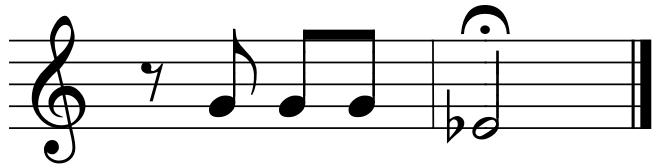
\includegraphics[scale=0.3]{imgs/symphonie5}
\end{figure}

\note \\
Be aware when using statically evaluated arguments that evaluable expression are evaluated during the \OSC{set} message processing, meaning that the value taken by such arguments depend on the INScore's state at this exact moment.

%===============================
\sublevel{Evaluating an ITLObject argument}

When processing an ITLObject argument, the evalutator will (for both statically or dynamically evaluated argument) try to extract a string from the given ITLObject. Passing a incorrect ITLObject identifier will cause the expression evaluation to fail. In general, evaluator can only make use of certain ITLObject (for guido expression evaluator, only symbolic notation object are useful), passing an ITLObject with a uninterpretable type will also cause the evaluation to fail.



\subsubsection*{Static evaluation}

Static ITLObject evaluation is an easy way to construct a score using its actual value, it can be considered as a weak recursion.
\pagebreak

\example\\
Creating a simple sample score, then duplicate it using \OSC{seq} and \OSC{par}:
\sample{/ITL/scene/score set gmn "[\{c,g\} e]";\\
/ITL/scene/score set gmn expr( seq score score);\\
/ITL/scene/score set gmn expr( par score score);
}
should produce the following output:\\
\begin{center}
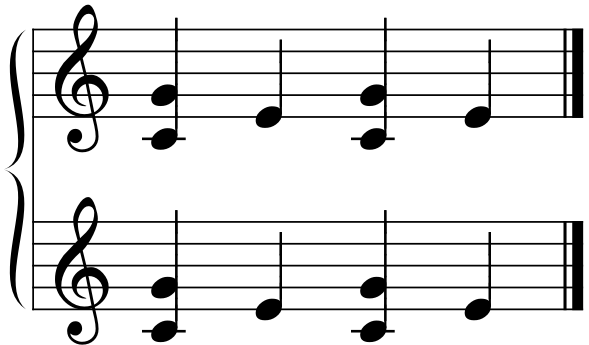
\includegraphics[scale=0.3]{imgs/seqpar}
\end{center}

\subsubsection*{Dynamic evaluation} (using \&)

Dynamic ITLObject evaluation is useful when manually re-evaluating the expression, the evaluation will be computed again accordingly to the value of the ITLObject at the time of the re-evaluation. This mechanisms also allow recursion. Keep in mind though, that a dynamic argument doesn't automatically update its value when its target's value change, update need to be manually triggered (which prevent any risk of infinite loop).

\example\\
Creating a sample score, then defining a recursive expression
\sample {/ITL/scene/score set gmn "[c d e f g a b]";\\
/ITL/scene/score set gmn expr( seq (tail \&score "[a]") (head \&score "[a]") );
}
Every time \OSC{/ITL/scene/score} is re-evaluated, its last note will be moved at the beginning of the score. (see Guido Expressions section for detail on operators).

\subsubsection*{Copy evaluation} (using \lowTilde)\\
It might be useful, when constructing expression using existing objects defined by expression, to not simply read the evaluated value of the object but to copy its entire expression. Looking back to the static evaluation example: one could want to define \OSC{/ITL/scene/score} as the duplication of an existing \OSC{/ITL/scene/simpleScore}, and still keep \OSC{score} up to date by re-evaluting  it when \OSC{simpleScore}'s value change... This is possible with copy evaluated arguments.

Indeed, on the first evaluation of these arguments (when processing the \OSC{set} message), their node in the expression will be replace by the entire expression of their targeted object. Evaluating a copy arguments is in fact expanding the expression using an already created one.

\example\\
Defining \OSC{/ITL/scene/score} as a \OSC{/ITL/scene/simpleScore} duplicated 4 times.
\sample{/ITL/scene/simpleScore set gmn "[a]";\\
\\
/ITL/scene/score set gmn expr( \&simpleScore );\\
/ITL/scene/score set gmn expr( seq \lowTilde score \lowTilde score);\\
/ITL/scene/score set gmn expr( par \lowTilde score \lowTilde score);\\
\\
/ITL/scene/simpleScore set gmn "[e \{c,g\} |]";
}
after re-evaluation, \OSC{/ITL/scene/score} should look like:\\
\begin{center}
 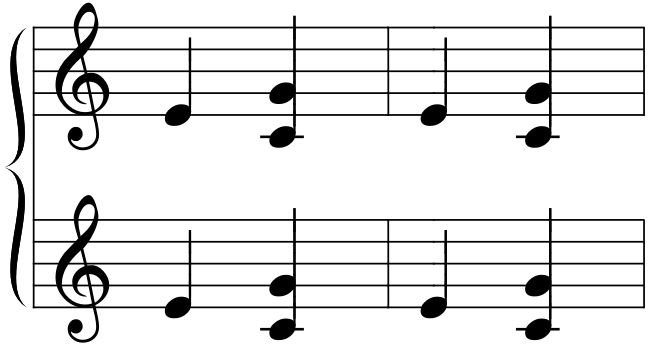
\includegraphics[scale=0.3]{imgs/seqparEnhanced}
\end{center}

Asking for \OSC{/ITL/scene/score} expression should return:

\begin{verbatim}
/ITL/scene/score expr
expr( par
       ( seq
          &simpleScore
          &simpleScore
       )
       ( seq
          &simpleScore
          &simpleScore
       )
    )
\end{verbatim}



%===============================
\sublevel{'expr' commands}

ITLObject defined using an evaluable expression gain access to these specific commands:

\begin{itemize}
\item \OSC{get expr}: return the actual expression tree state (including previously evaluated values between brackets for ITLObject and files)
\item \OSC{expr eval}: force the expression to re-evaluate
\item \OSC{expr renew}: clean the evaluated values and re-evaluate
\end{itemize}

Applied to an object which wasn't defined by an evaluable expression, all this commands will cause a bad argument error.
\smallbreak

The \OSC{renew} command reset the internal state of the evaluated variable, forcing the re-evaluation and update of every arguments in the expression. Be aware that the track of copy evaluated arguments is lost after the first evaluation, thus renewing an expression defined using copy evaluated arguments won't update these arguments to their targeted ITLObject expression. Though, static arguments added by the copy shall be renewed.
\pagebreak

\example\\
Lets compare the effect of renewing an expression with or without \lowTilde:
\begin{multicols}{2}


\sample{/ITL/scene/score set gmn "[a]";\\
\\
/ITL/scene/r set gmn expr(\&score);\\
/ITL/scene/r set gmn expr( par r r);\\
\\
/ITL/scene/score set gmn "[\{c,g\} |]";\\
/ITL/scene/r expr renew;
}
\OSC{r} evaluated expression is:
\begin{verbatim}
expr( par r r)
\end{verbatim}

so \OSC{r} should look like:
\begin{center}
 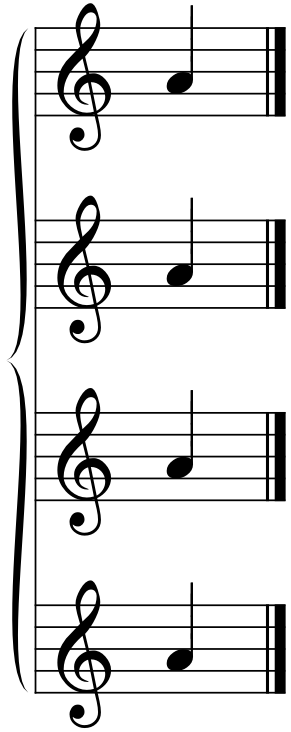
\includegraphics[scale=0.3]{imgs/renewWithout}
\end{center}

\columnbreak

\sample{/ITL/scene/score set gmn "[a]";\\
\\
/ITL/scene/r set gmn expr(\&score);\\
/ITL/scene/r set gmn expr( par \lowTilde r \lowTilde r);\\
\\
/ITL/scene/score set gmn "[\{c,g\} |]";\\
/ITL/scene/r expr renew;
}
\OSC{r} evaluated expression is:
\begin{verbatim}
expr( par &score &score)
\end{verbatim}

so \OSC{r} should look like:
\begin{center}
 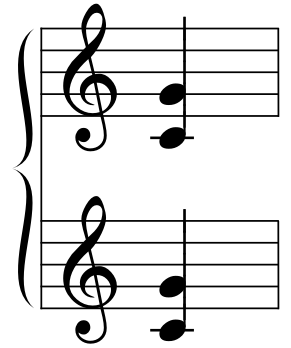
\includegraphics[scale=0.3]{imgs/renewWith}
\end{center}
\end{multicols}

\begin{itemize}
\item Without \lowTilde, renewing \OSC{r} means updating the two arguments \OSC{r} by its new value: \OSC{ "\{[a]\} \{[a]\}" }
\item With \lowTilde, renewing \OSC{r} means updating the value of \OSC{score}, thus \OSC{/ITL/scene/r expr reeval} would have had the same effect.
\end{itemize}

%===============================
\sublevel{newData event}

\OSC{newData} is triggered by any object when its value change (generally because of a \OSC{set} message). Neither trying to set an object to its actual value without changing its type, nor re-evaluating an object to its actual value will trigger newData.

Of course, the \OSC{newData} event can be used together with \OSC{reeval} to automatically update an object when the value of an other changes.

\example\\
Creating a copy of \OSC{score}, and automatise its update when \OSC{score} is changed
\sample{/ITL/scene/score set gmn "[c e]";\\
/ITL/scene/copy set gmn expr(\&score);\\
/ITL/scene/score watch newData (/ITL/scene/copy expr reeval);
}

To avoid infinite loop when using recursion, \OSC{newData} event is delayed of one event loop, meaning that, in the previous example, during the event loop that follow \OSC{score}'s modification, \OSC{score} and \OSC{copy} are different (\OSC{copy} has not been updated yet...).

\note\\
Because newData event is delayed, if \OSC{score} experiences multiple modifications during the same event loop (because multiple \OSC{set} messages have been sent together), only his final value will be accessible when newData will be actually triggered, however the event will be sent as many times as \OSC{score} have been modified.

\note {when automatising update}\\
For the reasons raised in the previous note, one should be very careful to delayed update when automatise \OSC{reeval} with \OSC{newData}. Indeed, in some extreme case, executing a script one line after an other won't have the same result as executing the all script at once!!

\example\\
Creating a "score buffer", storing every state adopted by \OSC{score}
\sample{/ITL/scene/score set gmn "[c]";\\
\\
/ITL/scene/buffer set gmn "[]";\\
/ITL/scene/buffer set gmn expr(seq \&buffer (seq "[|]" \&score));\\
/ITL/scene/score watch newData (/ITL/scene/buffer expr reeval);\\
\\
/ITL/scene/score set gmn "[e]";\\
/ITL/scene/score set gmn "[g]";\\
/ITL/scene/score set gmn "[\{c,e,g\}]";
}
Won't have the same result if run line by line, or the all script as once:
\begin{multicols}{2}

line by line:
\begin{center}
 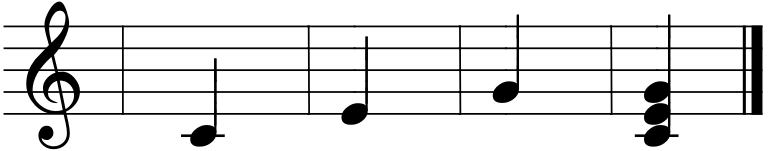
\includegraphics[scale=0.3]{imgs/autoSingleLine}
\end{center}

\columnbreak
all script at once:
\begin{center}
 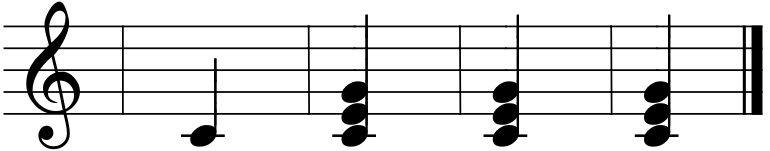
\includegraphics[scale=0.3]{imgs/autoAllScript}
\end{center}

\end{multicols}

To avoid such not deterministic behaviour, one should manually trigger \OSC{reeval} after each modification of \OSC{score}.

%===============================
%:Guido Expression
\toplevel{Guido Expressions}
\label{guidoExpr}

%===============================
\sublevel{Operators}

\printindex

\end{document}
